% !TeX root = 00Book.tex
\subsection{February: Hive Construction}

\begin{apiary}{Add candy block indicator}
    \path (4,6) pic{roof=candy};
    \path (4,4) pic{brood=8F};
    \path (4,2) pic{brood=8F};
    \path (4,0) pic{stand};

    \path (12,6) pic{roof=candy};
    \path (12,4) pic{brood=8F};
    \path (12,2) pic{brood=8F};
    \path (12,0) pic{stand};

    \path (20,6) pic{roof=candy};
    \path (20,4) pic{brood=8F};
    \path (20,2) pic{brood=8F};
    \path (20,0) pic{stand};
\end{apiary}

\subsubsection{Roof}

Space for a rapid feeder.


\subsubsection{Brood Box or Honey Super}

\begin{itemize}
    \item Chamfer the edges of the sides.
    \item Nail the rail in place, use long nose pliers so you don't hammer your fingers.
\end{itemize}

\subsubsection{Varroa Floor}

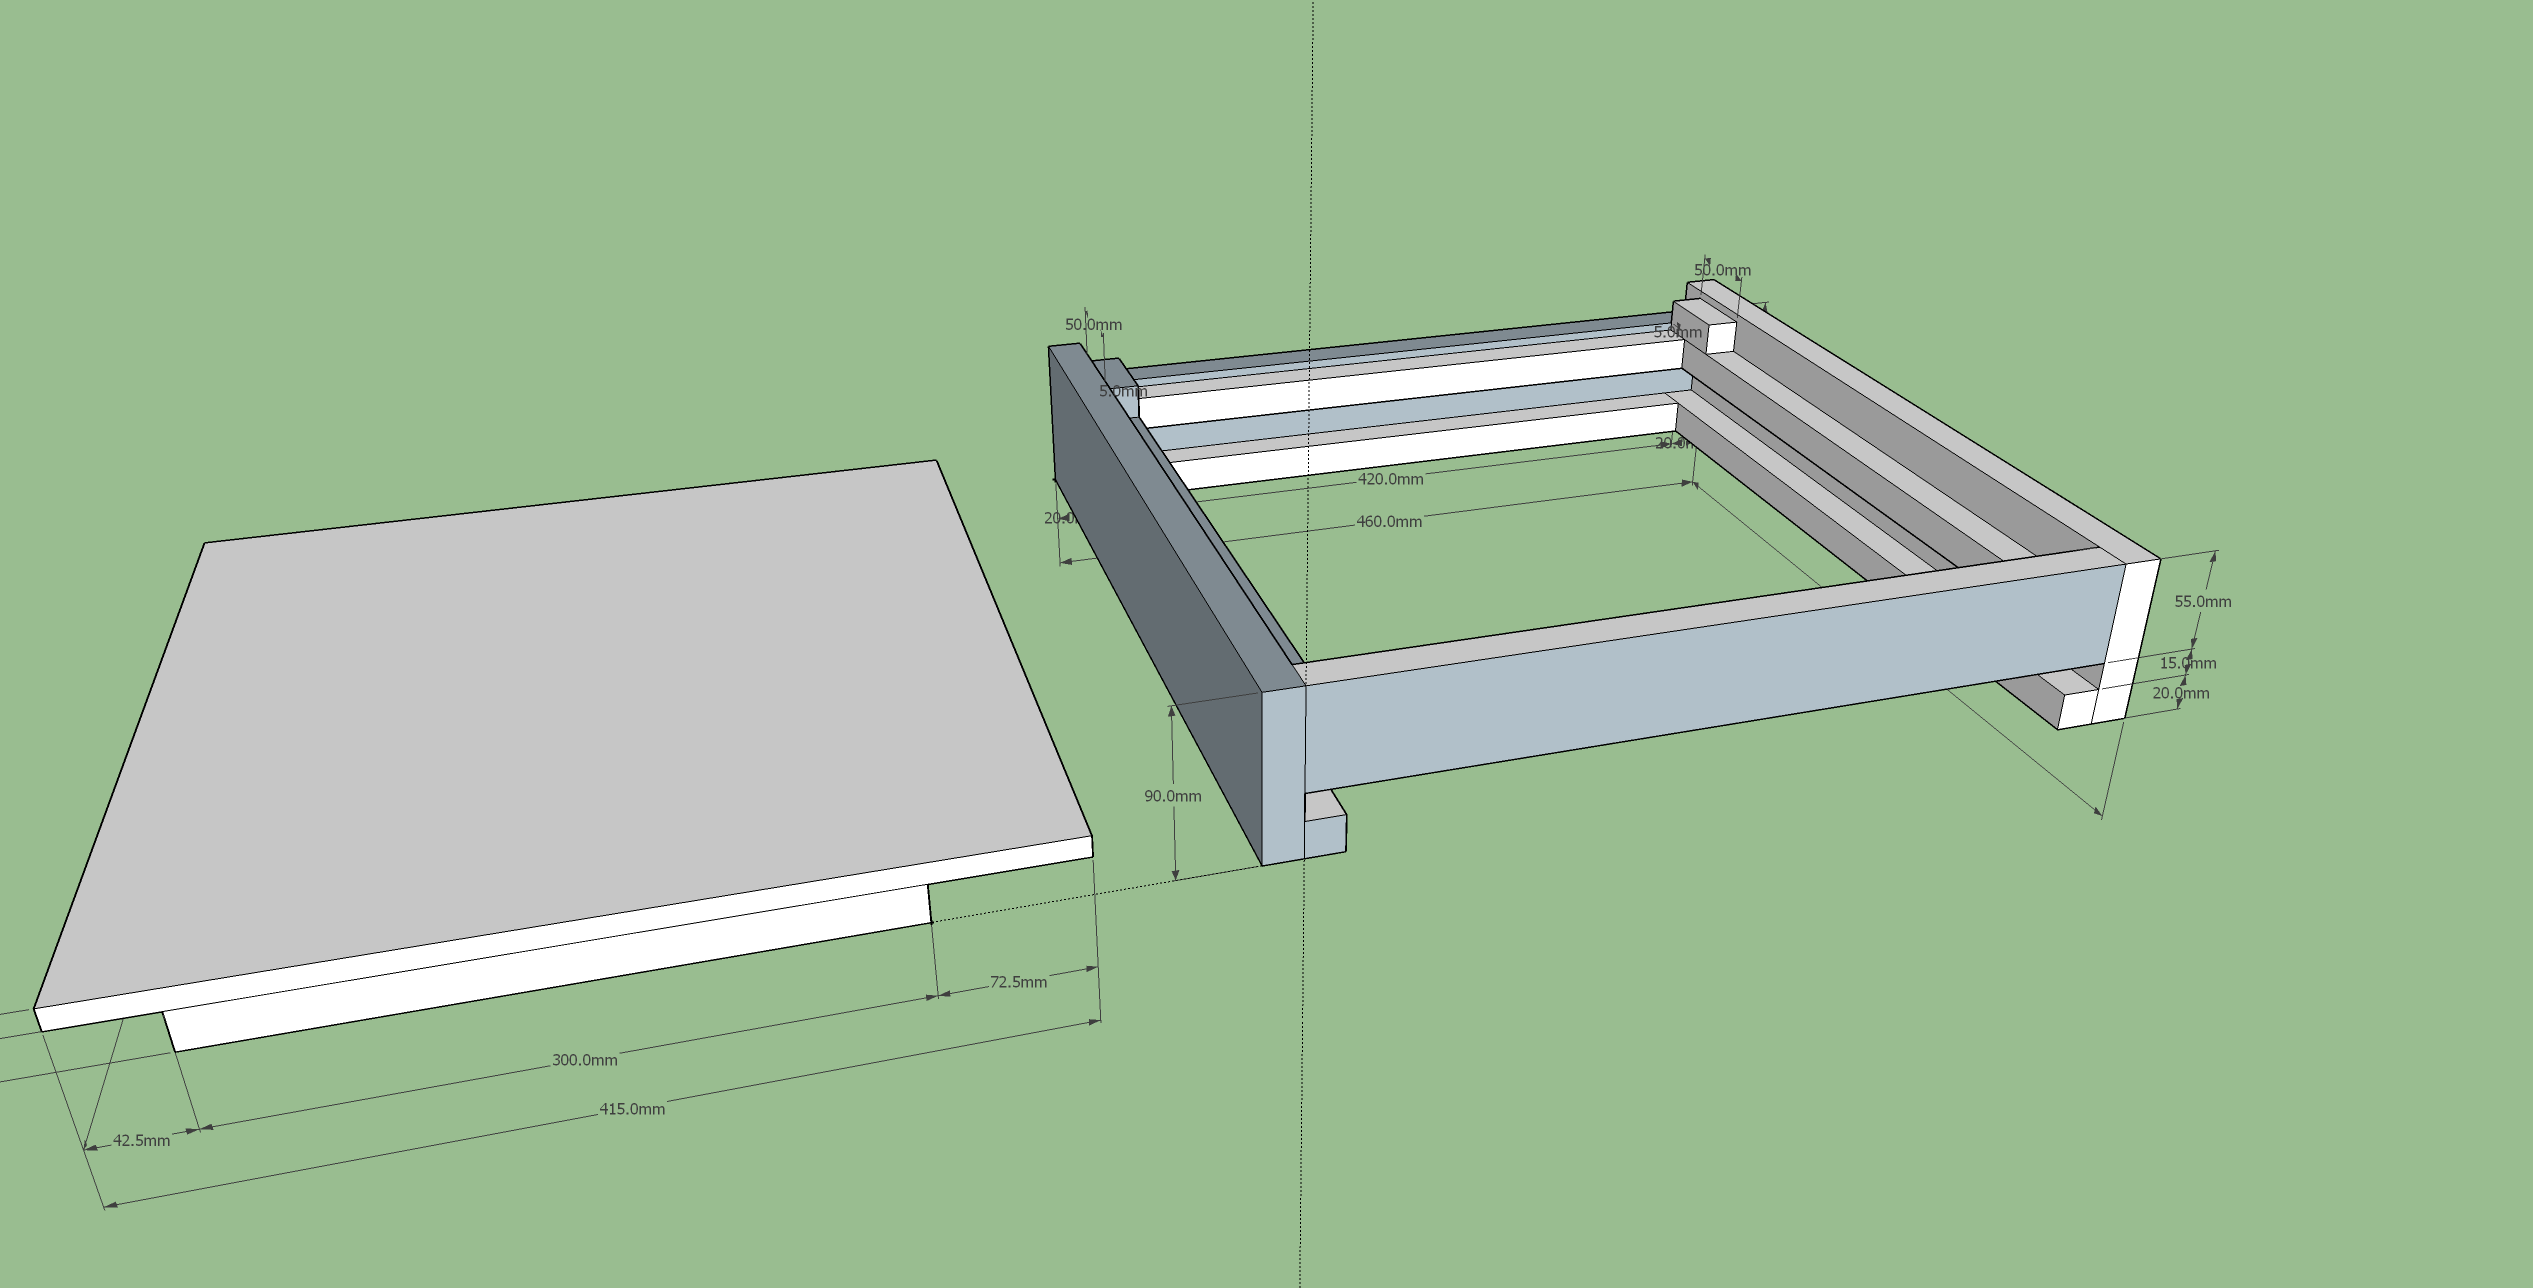
\includegraphics[width=0.9\textwidth]{../assets/varroa_floor.png}

\subsubsection{Entrance Block}

\subsubsection{Varroa Slide}

\subsubsection{Hive Stand}